\documentclass{article}
\usepackage[utf8]{inputenc}
\usepackage{amsmath}
\usepackage{graphicx}
\usepackage{float}

\title{COMP6245 : Lab 1 Report}
\author{Thanakorn Panyapiang(31446612)}

\begin{document}

\maketitle
\section{Linear Algebra}
\indent The command U @ U.T produces a 3x3 identity matrix because of a symmetric property of B. Since B is a symmetric matrix, all eigenvectors of B are othorgonal to each other. Therefore, U,a matrix which each column represents a unit eigenvector of B(according to numpy specification), is an \textit{orthorgonal matrix}.\\
\indent One property of an orthorgonal matrix is its transpose is equal to its inverse($A^T = A^{-1}$). Substituing this in the the command will get the result as follow:
\[U(U^T) = U(U^{-1})\]
\[U(U^{-1}) = I \] 

\maketitle
\section{Random Numbers and Univariate Distributions}
The distribution of uniform random samples with different numbers of samples and bins is as follow
\begin{center}
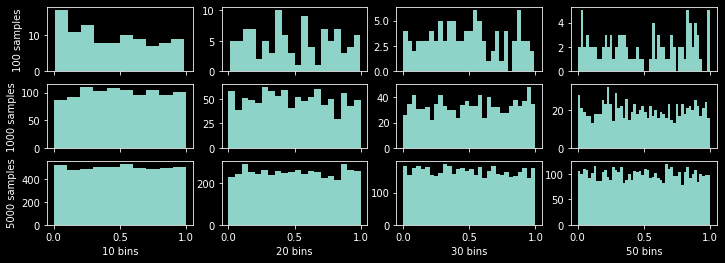
\includegraphics[scale=0.5]{uniform_random_numbers}
\end{center}
\indent It can be observed that, when the number of samples is high enough, data is distributed equally regardless of the number of bins which causes the variation within bin counts to be low.

\indent For samples drawn from a Gaussian distribution, the density of data, regardless of the number of samples, is higher when the value is close to mean and most of the data is located within 2 standard deviation(-2 to 2 in this case).
\begin{center}
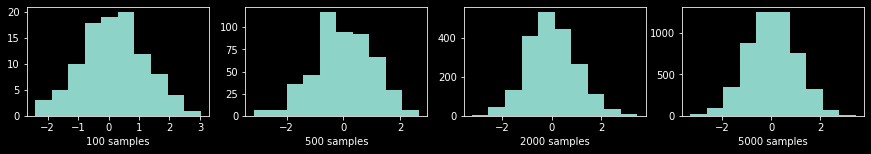
\includegraphics[scale=0.4]{gaussian_random_numbers}
\end{center}

In the samples where data is generated by summation of uniform random numbers, the distribution of data is similar to a Gaussian distribution. What can be clearly observed is that when the number of numbers to add/substract is increased, the distribution comes closer to a normal distribution.  
\begin{center}
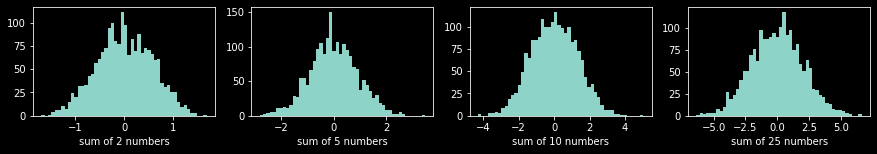
\includegraphics[scale=0.4]{sum_random_numbers}
\end{center}

\maketitle
\section{Uncertainty in Estimation}
The number of samples and the variance has an inverse relation for both sampling methods. Although the trends of variance over the number of samples are similar in both samplings, it can be noticed that uniform sampling has a significantly lower variance compare to Gaussian sampling.
\begin{center}
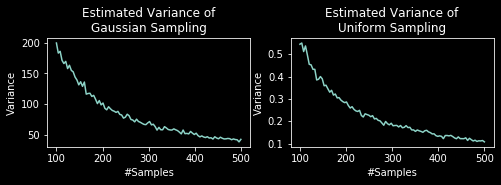
\includegraphics[scale=0.5]{estmd_variance}
\end{center}


\maketitle
\section{Bivariate Gaussian Distribution}
From the contour plot, $\overline{X}$ and $\overline{Y}$ are shifted by the value of the first and the second element of each matrix m as show in the figure below.
\begin{center}
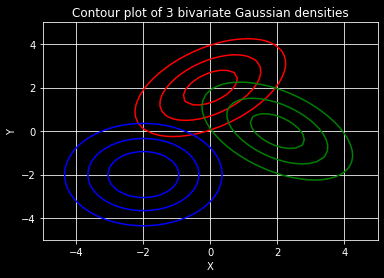
\includegraphics[scale=0.4]{contours}
\end{center}

For the covariance metrices, the diagonal elements affect the distribution scale of each variables while the off-diagonal elements change the correlation between two variables. From the graph, the size of all three contours is scaled up by 2 since diagonal elements of all metrices are 2. However, the correlations between X and Y are different from each other. The correleation is direct variation and inverse variation for the covariance matrix C1(red) and C2(green) respectively while on C3(blue) both variables are independent from each other.

\maketitle
\section{Sampling for Multivariate Gaussian Distribution}
The scatter plot of X and Y is shown in the figure below.
\begin{center}
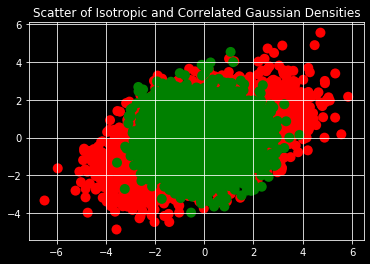
\includegraphics[scale=0.4]{scatter_of_isotropic}
\end{center}

Although X(green) and Y(red) have a normal distribution, their correlations of two variables are different. Both variables are independent from each other in X as illustrated in the shape of the scatter plot which is a normal circle. On the other hand, both variables are positively correlated(the density is high when the first and the second variable is close to each other) in Y. This is the result of a linear transformation of X by the cholesky factor of the covariance matrix $C = \begin{bmatrix}2 && 1\\1 && 2\end{bmatrix}$
\pagebreak

\maketitle
\section{Distribution of Projections}
The figure below shows the projected variance of Y as a function of $\theta$
\begin{center}
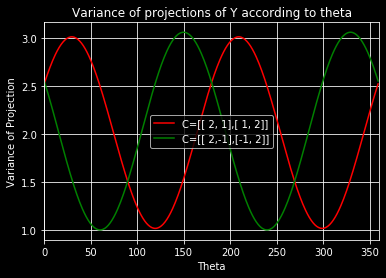
\includegraphics[scale=0.4]{variance_of_proj}
\end{center}
From the graph, it can be observed that the maximum and mininum variance of the projected data is 3 and 1 for both datasets, but the directions which gives the maximum and minimum variance are different.
Another thing that can be noticed is the eigenvalues of both covariance metrices are equal to the maximum and mininum projected variance. Also, when the data is projected into the direction of an eigenvector, the projected variance is equal to its corresponding eigenvalue. 
\end{document}